
% !TEX root = ../thesis.tex
\chapter{Data Collection}
\label{capitolo3}
\thispagestyle{empty}


In this chapter we present all the available datasets containing bot accounts, together with all the tools and methodologies used to collect the respective data. The final dataset contains:

\begin{itemize}
\item[\PencilRight]Data from already existing datasets
\item[\PencilRight]Data collected with different automated approaches
\item[\PencilRight]Hand-labelled data
\end{itemize}

\section{Tools}
Different tools were used in order to both collect the data and to enrich existing datasets. This stage was essential to gather additional features. Here we present all the instruments involved in this task.

\subsection{Tweepy}
Tweepy is a Python wrapper for the Twitter API.
Two main methods were used to collect all the default features of users and tweets:\\


\begin{tabular}{lll}
\centering	
	Method&Input&Output\\ \hline\hline
	API.get\_user&[id/user\_id/screen\_name]&User object\\
	API.user\_timeline&[user\_id][, count]&list of Status object\\ \hline\\
\end{tabular}

A User object contains all that features that describe the user's profile and his utilization of Twitter.
A Status object contains the details of a single tweet, such as the full text, number of retweets and replies.

\subsection{Botometer}
Botometer \cite{Botometer} checks the activity of a Twitter account and gives it a score based on how likely the account is to be a bot.

Authors et al \cite{Botometer} tested most classification algorithm with their dataset and highlighted Random Forest as their final classifier, since it gained the highest accuracy. Its accuracy was 98.42\% and 0.984 F1 measure \cite{Lee11sevenmonths}.

Botometer provides an API to check Twitter accounts authenticity.

\subsection{Hoaxy}
Hoaxy is a tool that visualizes the spreading of articles online. Articles can be found on Twitter, or other sources of misinformation and fact-checking.

For each fake news, Hoaxy plot a graph showing the users who tweeted the news on the nodes and the retweet activity on the edges. In this graph it is possible to figure out who invented the news and how the news spread.

Hoaxy only checks the news sources and compares them with a list of unreliable URLs.

\section{Datasets}

\subsection{Caverlee-2011}
The dataset et al. \cite{Lee11sevenmonths} is composed by content polluters, detected by a system composed of 60 social honeypots, which are Twitter accounts created to serve the purpose of tempting bots; and genuine accounts, randomly sampled from Twitter.
The authors observed the content polluters that used to interact with their honeypots, during a 7-months time-span. The accounts that weren't deleted, by the policy terms of the social platform, were clustered with the Expectation-Maximization algorithm for soft clustering. At the end of this process, the authors found nine different clusters, which were grouped in four main categories:

\begin{center}
	\begin{tabular}{>{\raggedright\arraybackslash}m{5.5cm}|>{\raggedright\arraybackslash}m{5.5cm}}
		\\Cluster&Description\\
		\hline\hline
		Duplicate Spammers & Accounts that post nearly the same tweets with or without links\\\hline
		Duplicate @ Spammers & Similar to the Duplicate Spammers, but they also use Twitter’s @ mechanism by randomly including a genuine account’s username\\\hline
		Malicious Promoters & These bots post tweets about marketing, business, and so on\\\hline
		Friend Infiltrators & Their profiles and tweets seem legitimate, but they mimic the mutual interest in following relationships\\\hline
	\end{tabular}
\end{center}

Each cluster has been manually checked, in order to asses its credibility.
Finally, 22,223 bots were included in the dataset.
For each content polluter, the authors collect the 200 most recent tweets, following and follower graph, and the temporal and historical profile information.

In order to collect genuine users too, 19,297 Twitter ids were randomly sampled and monitored  for three months, to see if they were still active and not suspended by the social platform moderation service.

The authors subsequently built a classifier framework trained on their dataset, which uses crafted features grouped in four clusters:
User Demographics (\textbf{UD}), User Friendship Networks (\textbf{UFN}), User Content (\textbf{UC}) and User History (\textbf{UH}).
After testing several classification algorithms, the most performing algorithm was Random Forest with boosting sampling, which accomplished 98.62\% of accuracy, 0.986 of F1-measure and 0.995 in the AUC score.

\subsection{Cresci-2017}
Cresci Dataset et al. \cite{Cresci} is composed of genuine accounts and bots. In this dataset there is a further differentiation of bots in sub-classes, which are precisely marked according to different categories.

\tiny
\begin{center}
\begin{tabular}{lllll}
	Dataset&Description&\#Users&\#Tweets&Year\\ \hline\hline
	genuine accounts&
	verified accounts that are human-operated&
	3,474&
	8,377,522
	&2011\\
	social Spam-Bots \#1&
	retweeters of an Italian political candidate&
	991&
	1,610,176&
	2012 \\
	social Spam-Bots \#2&
	spammers of paid apps for mobile devices&
	3,457&
	428,542&
	2014 \\
	social Spam-Bots \#3&
	spammers of products on sale at	Amazon&
	464&
	1,418,626&
	2011 \\
	traditional Spam-Bots \#1&
	training set of spammers used by Yang \cite{Yang}&
	1,000&
	145,094&
	2009 \\
	traditional Spam-Bots \#2&
	spammers of scam URLs&
	100&
	74,957&
	2014 \\
	traditional Spam-Bots \#3&
	automated accounts spamming job offers&
	433&
	5,794,931&
	2013 \\
	traditional Spam-Bots \#4&
	automated accounts spamming job offers&
	1,128&
	133,311&
	2009 \\
	Fake-Followers&
	accounts inflating followers of other accounts&
	3,351&
	196,027&
	2012 \\ \hline\\
	
\end{tabular}
\end{center}

\normalsize
\begin{itemize}
	\item \textbf{Genuine accounts} are those users who correctly answered to a simple question, posed in natural language, so they represent accounts with no automation.
	\item  During Rome majoral election in 2014, one of the candidates used a set of automated accounts to publicize his policies. These accounts were gathered to be part of the \textbf{Social Spam-Bots \#1}.
	\item \textbf{Social Spam-Bots \#2} are accounts that promotes mobile app, using popular hashtags for months.
	\item  \textbf{Social Spam-Bots \#3} promotes products on sale on Amazon, by tweeting products URL and descriptions.
\end{itemize}
All these accounts were manually checked to verify their automated nature.

\begin{itemize}
	\item The \textbf{Traditional Spam-Bots \#1} dataset is the training set used in \cite{Yang}.
	\item \textbf{traditional Spam-Bots \#2} are users that mention other users in tweets containing scam URLs. They usually invite users to claim a prize.
	\item \textbf{Traditional Spam-Bots \#3} and \textbf{traditional Spam-Bots \#4} are bots that continuously tweet job offers.
	\item \textbf{Fake-Followers} are account involved in increasing popularity of other users. In order to collect them, Cresci et al. \cite{Cresci} bought followers from fastfollowerz.com, intertwitter.com and twittertechnology.com.
\end{itemize}

The intent of this project was to find a methodology useful to detect sophisticated Spam-Bots on Twitter. This novel category differs from the traditional Spam-Bot type, due to the ability of those content polluters to mimic the human interactions on the social platform. The authors et al. \cite{Cresci} relied on both crowdsourcing and machine learning experiments to compare the accuracy of the detection of such Spam-Bots. The experiments highlighted the difficulty of detecting this new wave of Spam-Bots, even with the help of human annotators.


\subsection{Varol-2017}
The Varol dataset et al. \cite{Varol} contains a list of Twitter accounts, labeled as bots (1) or humans (0).

The construction of this dataset starts with the identification of a representative sample of users, by monitoring a Twitter stream for 3 months, starting in October 2015. Thanks to this approach it is possible to collect data without bias; in fact other methods like snowball (a technique that nominee new samples, starting from the social networks of an initial pool of users) or breadth-first (a graph exploration technique) need an initial users set.
During the observation window about 14 million user accounts were gathered. 
All the collected users had to have at least 200 tweets in total and 90 tweets during the three month observation (about one tweet per day).

Using the classifier trained on the honeypot dataset in \cite{Lee11sevenmonths}, the authors et al. \cite{Varol} computed the classification scores for each of the active accounts, obtaining 0.85 in the AUC metric score, a lower score then the one obtained, by the same model, on the honeypot's data (0.95 AUC). This difference was justified by the lower ages of the manually annotated bots, with respect to the ones collected by the social honeypots.
Then the samples were grouped by their score and 300 accounts from each bot-score decile were randomly selected. 
The 3,000 extracted accounts were manually labeled by volunteers. The authors analyzed users profile, friends, tweets, retweets and interactions with other users. Then a label was assigned to each user.
Of course the final decision is conditioned to personal opinion.

\subsection{BotBlock}
Botblock (https://github.com/dansarie/Botblock) is a Twitter block list (on Twitter users can use these lists to block any interaction with the accounts listed) containing the user ids of a large number of known porn bot accounts. 
They are mainly used to aggressively market porn sites.

\section{Unsupervised labeling of datasets}
At first try, we wanted to understand if different kinds of bots were easy to distinguish, using their profile features only. We didn't know what kinds of bots populate Twitter for the most. So, an unsupervised approach could have helped us to highlight different categories. We relied expectations on clustering techniques, hoping to get a solid help in automatizing the labeling process of the data.\\
We used the Varol dataset \cite{Varol}, that contains a plain list of bots and humans.\\
It was not possible to use all the data, because we needed to scrape from the web all the possible features and some of the listed accounts were already been deleted. So, for this work, we had to consider only those accounts that were still active.\\
The first step was the knee-elbow analysis based on a hierarchical clustering with single linkage and euclidean distance. We used this technique in order to determine the optimal number of clusters. The data must had been preprocessed and cleaned.\\
Here we illustrate what kind of pre-process operations were performed for that purpose; features marked with '---' don't need to be preprocessed:

\small
\begin{center}
	\begin{tabular}{lll}
		\\feature&type&preprocess operation\\
		\hline\hline
		id&int&delete\\
		name&str&replace with len(name)\\
		screen\_name&str&replace with len(screen\_name)\\
		statuses\_count&int&---\\
		followers\_count&int&---\\
		friends\_count&int&---\\
		favourites\_count&int&---\\
		listed\_count&int&---\\
		url&str&replace with hasUrl (0/1)\\
		lang&str&one hot encoding\\
		time\_zone&str&one hot encoding\\
		location&str&one hot encoding\\
		default\_profile&int&replace with hasDefaultProfile (0/1)\\
		default\_profile\_image&boolean&boolean to int (0/1)\\
		geo\_enabled&boolean&boolean to int (0/1)\\
		profile\_image\_url&str&delete\\
		profile\_use\_background\_image&boolean&boolean to int (0/1)\\
		profile\_background\_image\_url\_https&str&delete\\
		profile\_text\_color&str&delete\\
		profile\_image\_url\_https&str&delete\\
		profile\_sidebar\_border\_color&str&delete\\
		profile\_background\_tile&boolean&boolean to int (0/1)\\
		profile\_sidebar\_fill\_color&str&delete\\
		profile\_background\_image\_url&str&delete\\
		profile\_background\_color&str&delete\\
		profile\_link\_color&str&delete\\
		utc\_offset&int&delete\\
		is\_translator&boolean&boolean to int (0/1)\\
		follow\_request\_sent&int&delete\\
		protected&boolean&boolean to int (0/1)\\
		verified&boolean&boolean to int (0/1)\\
		notifications&boolean&delete\\
		description&str&replace with hasDescription (0/1)\\
		contributors\_enabled&boolean&boolean to int (0/1)\\
		following&boolean&delete\\
		created\_at&str&string to int (year)\\\hline\\
	\end{tabular}
\end{center}

\normalsize
\clearpage

Since we didn't know how many categories of bots were listed in this dataset, the first step consisted in understanding which was the optimal number of clusters to look for. To achieve that goal, we applied \textit{hierarchical clustering}. This is a method of cluster analysis which build a hierarchy of clusters. The results of hierarchical clustering are usually presented in a dendrogram, that illustrates the arrangement of the clusters produced.
In figure (\ref{fig:dendogram}) you can see the dendogram of the algorithm.


\begin{figure}
	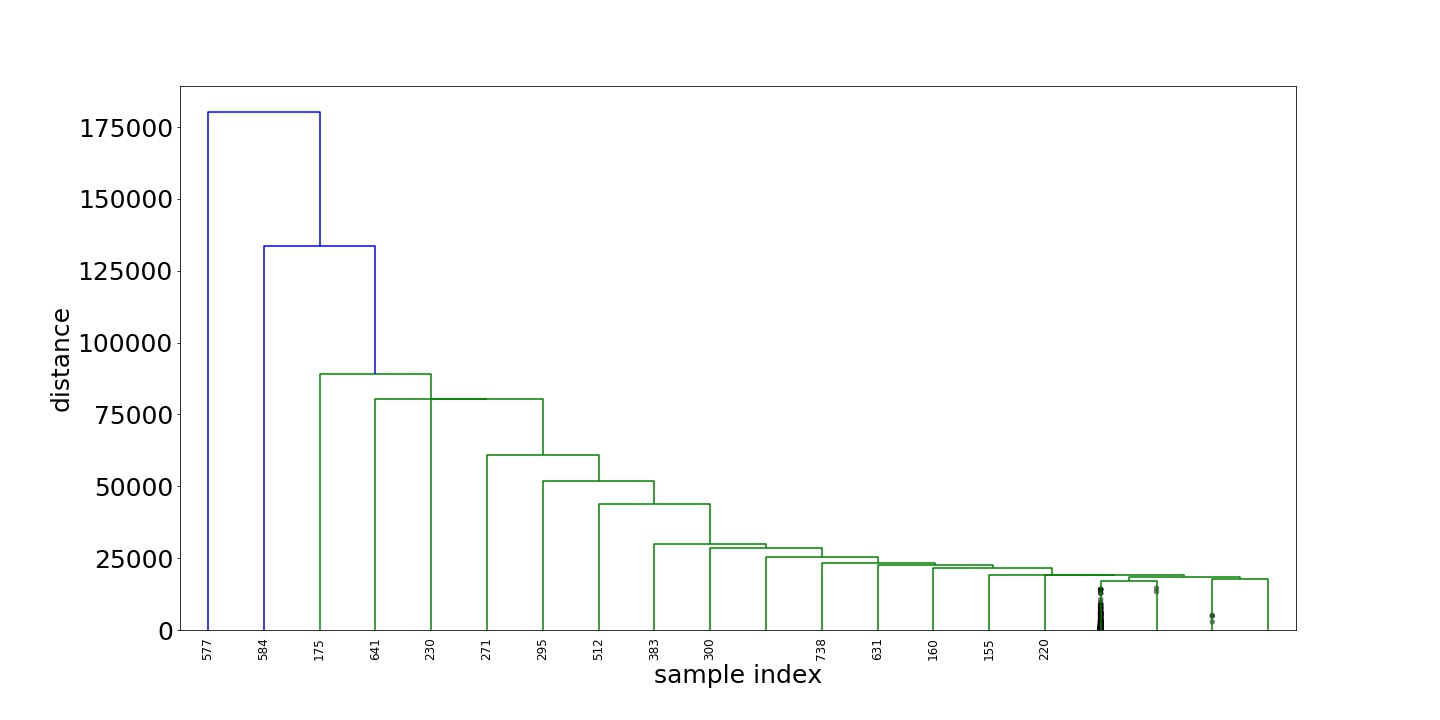
\includegraphics[width=\linewidth]{chapter3/figure/dendogram.jpg}
	\caption{Hierarchical Clustering Dendrogram (truncated to the last 20 merged clusters)}
	\label{fig:dendogram}
\end{figure}

In order to select the optimal number of clusters, we plotted the knee-elbow figure (\ref{fig:kneeelbow}). It shows the variation of WSS (within cluster sum of squares) and BSS (between cluster sum of squares) as the number of clusters increase.\\

\begin{figure} [htp!]
	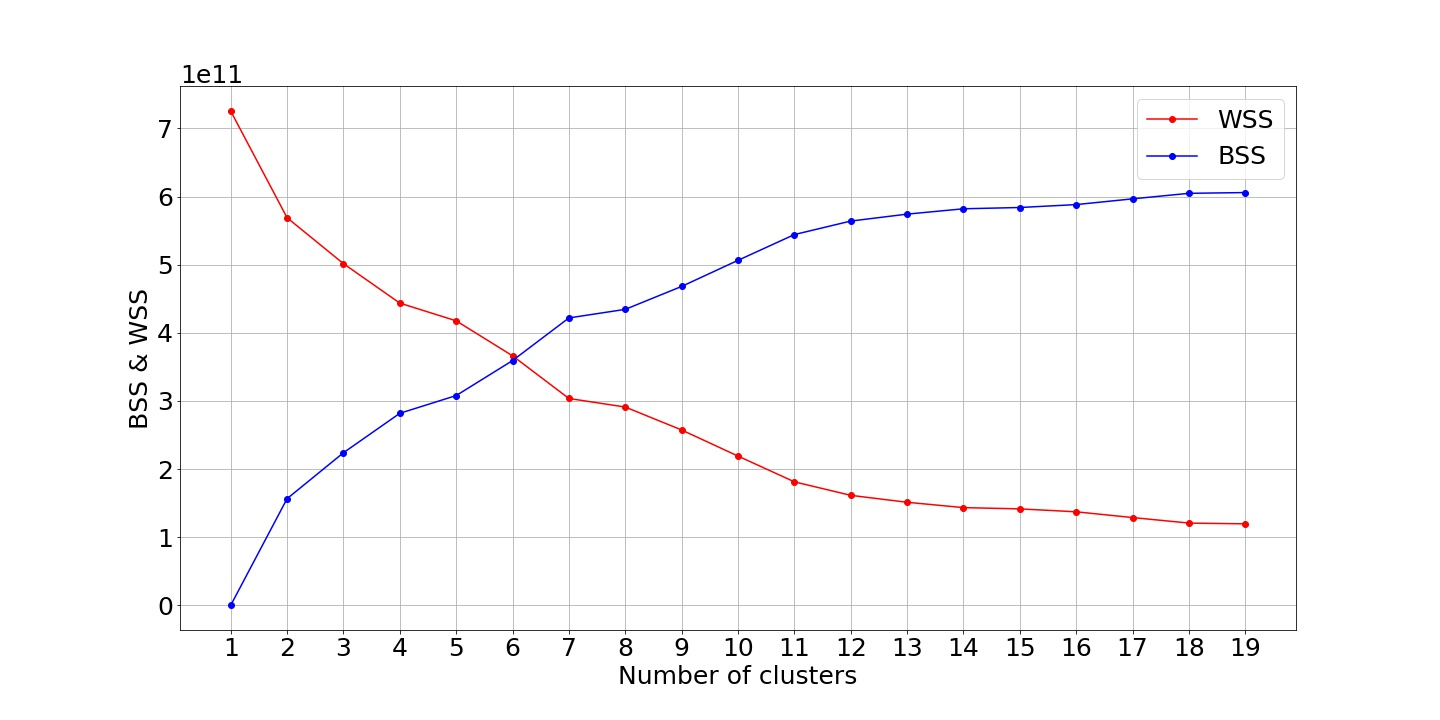
\includegraphics[width=\linewidth]{chapter3/figure/kneeelbow.jpg}
	\caption{Hierarchical Clustering - knee-elbow}
	\label{fig:kneeelbow}
\end{figure}

\newpage
It is clear that there are no well-defined elbows or knees, both curves seems to be ''smooth'', so it were hard to pick a reasonable k (number of clusters) for the algorithms to come.

Then we tried another approach. We applied the \emph{K-means} algorithm and we plotted the elbow method (\ref{fig:elbow}). In this figure there is an elbow between k=3 and k=4, so the most accurate solution were represented by four clusters.

\begin{figure}
	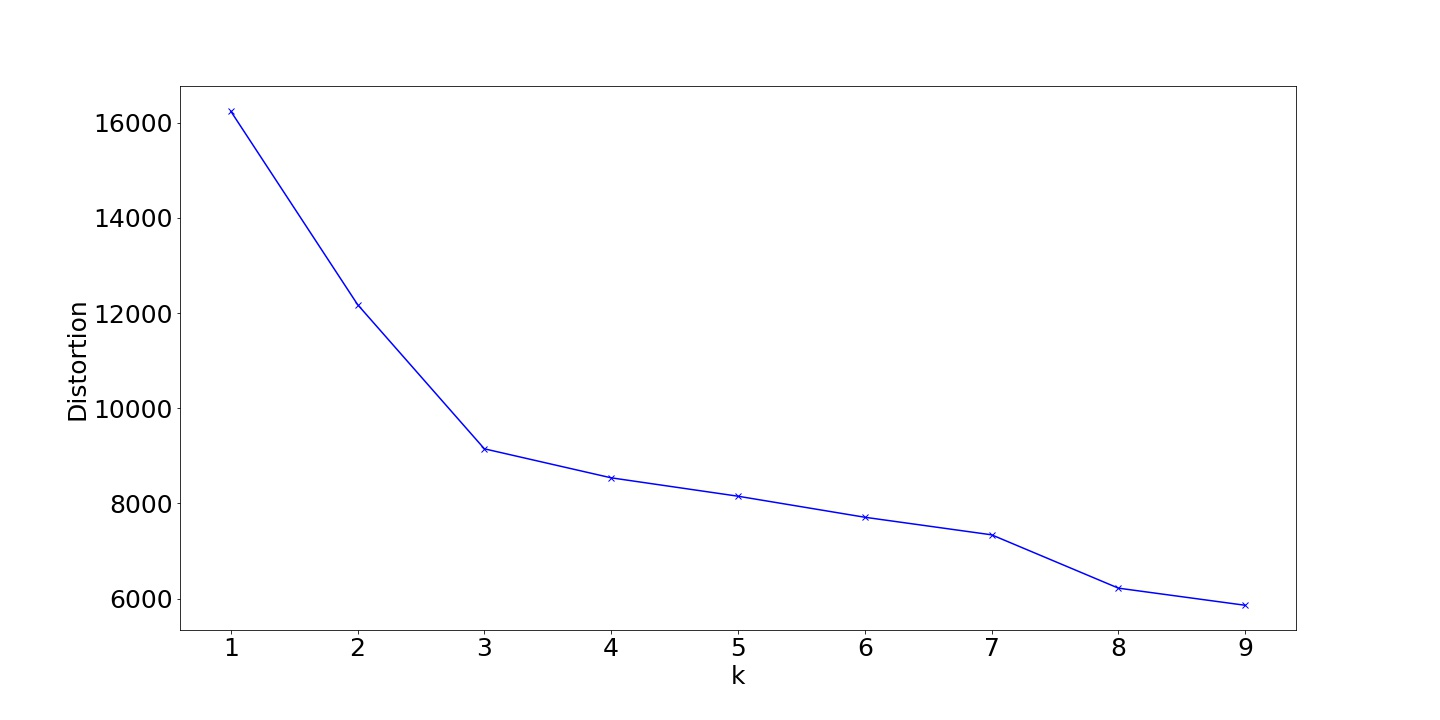
\includegraphics[width=\linewidth]{chapter3/figure/elbow.jpg}
	\caption{The Elbow Method showing the optimal k}
	\label{fig:elbow}
\end{figure}


As this process came to an end, we manually inspected the resulting clusters.

\begin{center}
	\begin{tabular}{ll}
	\\cluster&size\\
	\hline\hline
	cluster 1&82\\
	cluster 2&648\\
	cluster 3&2\\
	cluster 4&16\\\hline
	\end{tabular}
\end{center}

Cluster 2 contains most of the samples, while the others have fewer elements.
We observed the Twitter profile of all the elements belonging to cluster 1, 3, 4 and a small sample of profiles for cluster 2.

Unfortunately there was no behavioural correlation among accounts in the same cluster, they just had similar values in the default features (i.e. number of followers, number of tweets, etc). So this technique didn't seem to fit the speeding up of the labeling process, nor to create useful features for a classifier.

\section{Supervised labeling of datasets}
The clustering approach did not help us, but the manual inspection of the clusters allowed us to get in touch with some existing bots, making us understand which categories of bots are most common on the social network. In particular we detected 4 main classes:
\begin{itemize}
	\item[\PencilRight]NSFW bots
	\item[\PencilRight]News-Spreaders
	\item[\PencilRight]Spam-Bots
	\item[\PencilRight]Fake-Followers
\end{itemize}

We started with a hand-labeling of the Varol dataset \cite{Varol}. For each account we analyzed its profile and tweets and we assigned it a label according to the categories we identified. We have faced some unexpected behaviors among bot accounts, that didn't fit the above-mentioned categories. For example, we found harmless bots, whose goal was to improve their ability of formulating sentences. In these cases, they were temporarily signed as ''general purpose''.

We also found genuine users, who we thought  had been incorrectly added to the dataset.
This task resulted into the collection of the following bots:

\begin{center}
	\begin{tabular}{ll}
		\\category&labeled account\\
		\hline\hline
		NSFW&31\\
		News-Spreader&71\\
		Spam-Bots&418\\
		Fake-Followers&5\\
		general purpose&63\\
		genuine&104\\\hline\\		
	\end{tabular}
\end{center}

\emph{''General purpose''} accounts are sometimes bots with no goal, they aim to emulate human behavior and often they were recognizable just because their description informs other users about their own nature.

Sixtythree users were not enough to represent a class and it was not possible to find a large list of those accounts who act like them, so we added all these ids to the ''genuine'' group. Even if this choice brought some noise to our data (since we added some bots in a humans dataset), it allowed us to provide our data more heterogeneity.

\emph{''NSFW''} accounts are only thirtyone elements, anyway the problem of pornography is a known issue on Twitter. In \cite{Varol} they clusterize users too. ''These bot clusters exhibit some prominent properties: cluster C0, for example, consists of legit-looking accounts that are promoting themselves (recruiters, porn actresses, etc.)'' \cite{Varol}.
This kind of users are often banned by Twitter, so it is likely that the accounts that we were not able to scrape, used to belong to this category.
Therefore we firmly believed that obtaining further accounts of this class was fundamental.

Finally it is clear that even Fake-Followers were few, since they were not considered in the research by Varol, but they are important in the Cresci one \cite{Cresci}, so we decided to expand this category too.

All these samples were not enough to train a classifier, hence we needed to collect more data. We performed this task by focusing on one category at a time.

\subsection{NSFW}
\emph{Not safe for work} is a tag used on internet to mark all that URLs, web pages, e-mails that contain nudity, intense sexuality, profanity or violence. In particular we wanted to collect a specific sub-category: the pornbots. In order to collect them, we used the BotBlock dataset.

BotBlock contains thousands of pornbot ids. We wanted to gather about 6,000 samples, an amount that would have been enough for the final dataset, with regards to its balance.
Since they were sorted according to their creation date, we shuffled the whole list. Then, using the Twitter API, we looked for accounts that weren't deleted yet. 
We needed to scrape profile features and tweets, so we couldn't consider banned accounts. The user list was initially shuffled to allow us to collect users with different ages. This emerged as a very useful step, because we gathered both more long-lived accounts and more explicit accounts (which probably have shorter lives). We finally obtained 6,605 accounts and 198,378 tweets.
\subsection{News-Spreaders}
Many bots on Twitter are News-Spreaders. The goal of these users is to spread politics, sports or other news. Often their behavior is not harmful, they just retweet statuses from newspapers accounts. However, there are users created to diffuse fake news. In the last few years Twitter has been used to boost politics propaganda. During elections or political campaigns, ad hoc accounts are created to divulgate specific political idea.

As a recent study highlighted, about 80\% of these ''pre-elections bots'' are still alive \cite{Disinformation}. It is possible that some of them have been included in our News-Spreader dataset.

We started gathering these ids by exploring Hoaxy.
We used two different approaches.
\begin{figure}[htp]
	\centering
	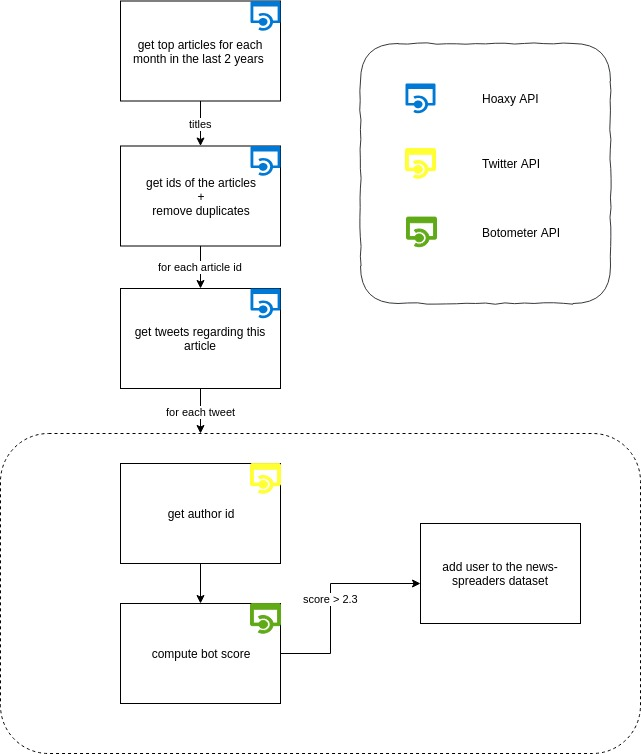
\includegraphics[width=\columnwidth]{chapter3/figure/news-spreader.jpg}
	\caption{Collection of News-Spreading bots, approach 1}
	\label{fig:News-Spreaders}
\end{figure}
The first way (in figure \ref{fig:News-Spreaders}) consisted in collecting the twenty top popular fake news, for each month, in the last two years. We performed this task using the Hoaxy APIs. Thanks to this service, we obtained all the tweet ids that have spread the considered claim. With the official Twitter APIs we collected all the users involved in this spreading activity. We finally passed all these accounts to the Botometer API, since many of the retrieved users were humans.

We set a threshold, in order to classify a user as a bot. That threshold is 2.3 due to the willingness of including some false positives in our data, increasing the heterogeneity in their behaviors and the challenge level for the classifiers. We think that a high intra-homogeneity among classes could lead the models to perform well on the training data, but worse over unseen ones; so we set a lower threshold to lower the intra-homogeneity of the News-spreaders dataset.

The second approach just consisted in collecting the most popular News-Spreaders according to Hoaxy. In consistency with the mentioned threshold, profiles with a Botometer score lower then 2.3 were still discarded.

Finally we checked every profile added to this dataset and removed all those users who didn't tweet enough statuses to be included in this class. This hand-made analysis made us know that there are no bots who only spread fake news. Usually they tweet a lot of verified news and some fake ones, to keep their credibility.
We reached 3,590 accounts and 333,699 tweets.

\subsection{Spam-Bots}
As seen before, Spam-Bots were already collected in the work of Cresci et al. \cite{Cresci}. Authors allowed us to access their dataset, so we obtained the Spam-Bots list by sampling their data. Due to homogeneity reasons, we needed to perform scraping again, since we needed different features compared to the available ones.
We selected users from:
\begin{itemize}
	\item[\PencilRight]traditional Spam-Bots 1
	\item[\PencilRight]social Spam-Bots 2
	\item[\PencilRight]social Spam-Bots 3
\end{itemize}

We chose this categories because they contain the most popular kinds of Spam-Bots, that are the ones who advertise products, services or mobile applications. We ignored \emph{''social Spam-Bots 1''}, since they are italian News-Spreaders and \emph{''traditional Spam-Bots 3 and 4''}, since we retrieved enough job-offer spammers during the hand-made labeling. If we had stored too many bots of this category, we would not have been able to generalize on generic Spam-Bots. Finally we gathered 4,943 accounts and 458809 tweets.

\subsection{Fake-Followers}
The collection of this class was quite easy. We initially performed scraping of the data collected by the work of Cresci et al. \cite{Cresci}. Many of these accounts had already been banned, so we could not collect their features. In order to enrich our dataset, we created a new Twitter account (figure \ref{fig:dibebot}). Then we bought Fake-Followers from two different services:
\begin{itemize}
	\item[\PencilRight] instakipci.com/
	\item[\PencilRight] rantic.com/buy-legit-twitter-followers/
\end{itemize}

\emph{Instakipci} provides low-quality followers. Usually they have no tweets, no followers and a they have a lot of followings.

\emph{Rantic}, on the other hand, ensures more realistic followers. They seem to have a real network of friends and, sometimes, they tweet too.

By using both services, we gathered a more miscellaneous dataset.
We collected 6,307 users and 41,683 tweets for about 20\$.
\begin{figure}
	\centering
	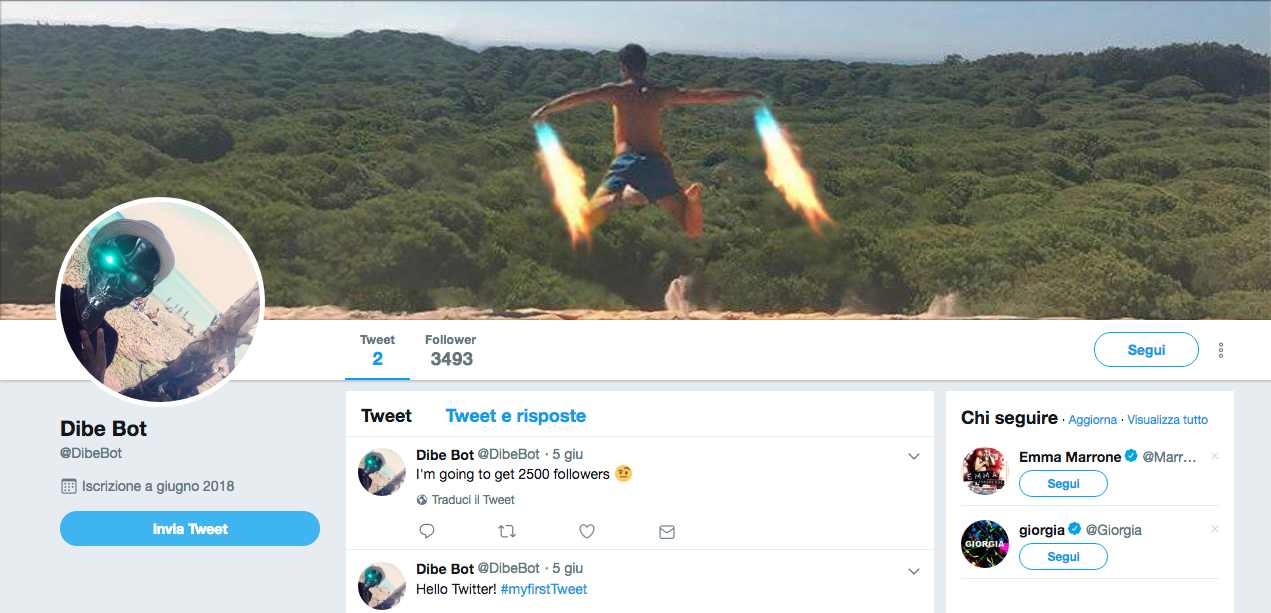
\includegraphics[width=\columnwidth]{chapter3/figure/dibebot.png}
	\caption{Collection of Fake-Followers bots}
	\label{fig:dibebot}
\end{figure}

\subsection{Genuine}
Finally we needed genuine accounts. We used again the Cresci dataset \cite{Cresci} and we filled it with all the Varol users labeled as humans. We again performed scraping on the existing accounts and we collected 3,661 users and 263,240 tweets in total.
Morover, we gathered all the Genuine users from the Caverlee dataset \cite{Lee11sevenmonths}. these are many more than other classes, but they will be necessary for a future classification between bots and humans. We perfomed scraping and we were able to obtain 15,701 users and 1,278,852 tweets.

\subsection{Bots}
We needed a set of unlabeled bots in order to train a binary classifier, that is able to classify bots and humans. We again scraped the Caverlee dataset \cite{Lee11sevenmonths} and we gathered 15,539 and 1,276,457 tweets.

\subsection{Final Datasets}
\label{sec:dataset}
At the end of the collection, we set up two datasets. The first one is the \textit{multi-class} dataset, that contains only bots labeled according to the type of threat, its composition is the following:

\begin{center}
\begin{tabular}{lll}
	\\category&\# users&\# tweets\\
	\hline\hline
	NSFW&6,605&198,378\\
	News-Spreader&3,590&333,699\\
	Spam-Bots&4,943&458,809\\
	Fake-Followers&6,307&41,683\\\hline\\	
\end{tabular}
\end{center}

The second dataset is the \textit{Binary} dataset, containing bots and genuine users.

\begin{center}
	\begin{tabular}{lll}
		\\category&\# users&\# tweets\\
		\hline\hline
		Bots&15,539&1,276,457\\
		Genuine&15,701&1,278,852\\\hline\\	
	\end{tabular}
\end{center}

\newpage
\section{Descriptive statistics of datasets}
As the collection of the data was completed, we explored our final multi-class dataset. In this section we will only focus on different categories of bots, which is the most interesting part.

A first look (\ref{fig:bubble}) shows us how many user accounts we collected (y axis) for each class and how many tweets we could scrape (diameter). It is easy to observe that Fake-Followers and NSFW bots have fewer tweets than the others, while News-Spreaders have a lot of tweets, but we collected fewer profiles.
\begin{center}
	\begin{tabular}{ll}
		\\category&target id\\
		\hline\hline
		NSFW&0\\
		News-Spreader&1\\
		Spam-Bots&2\\
		Fake-Followers&3\\\hline\\		
	\end{tabular}
\end{center}


\begin{figure}[htp!]
	\centering
	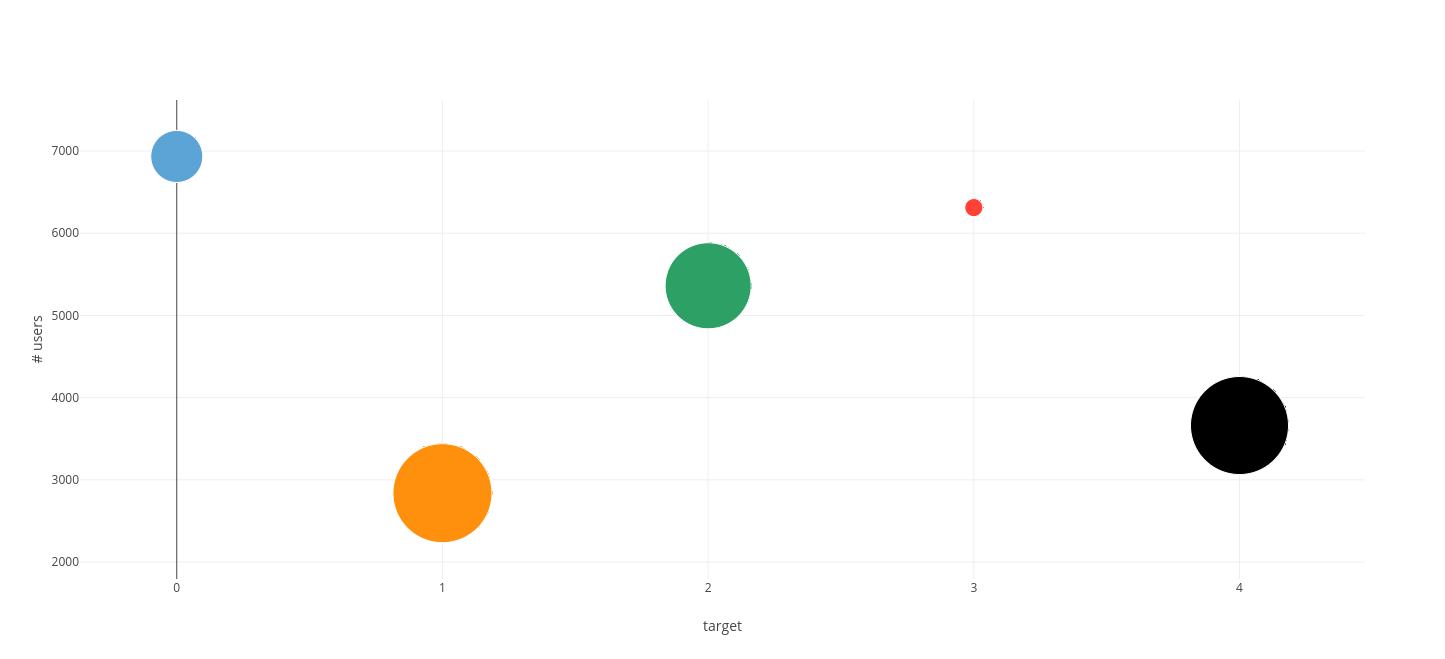
\includegraphics[width=\columnwidth]{chapter3/figure/bubble.png}
	\caption{Users amount and tweets}
	\label{fig:bubble}
\end{figure}
\newpage
Then we plotted the heatmap of the correlation matrix (\ref{fig:heatmap}). We wanted to undestand if some feature was more useful to predict the correct target. This plot suggested us that there were no features highly correlated to the target.
\begin{figure}[htp!]
	\centering
	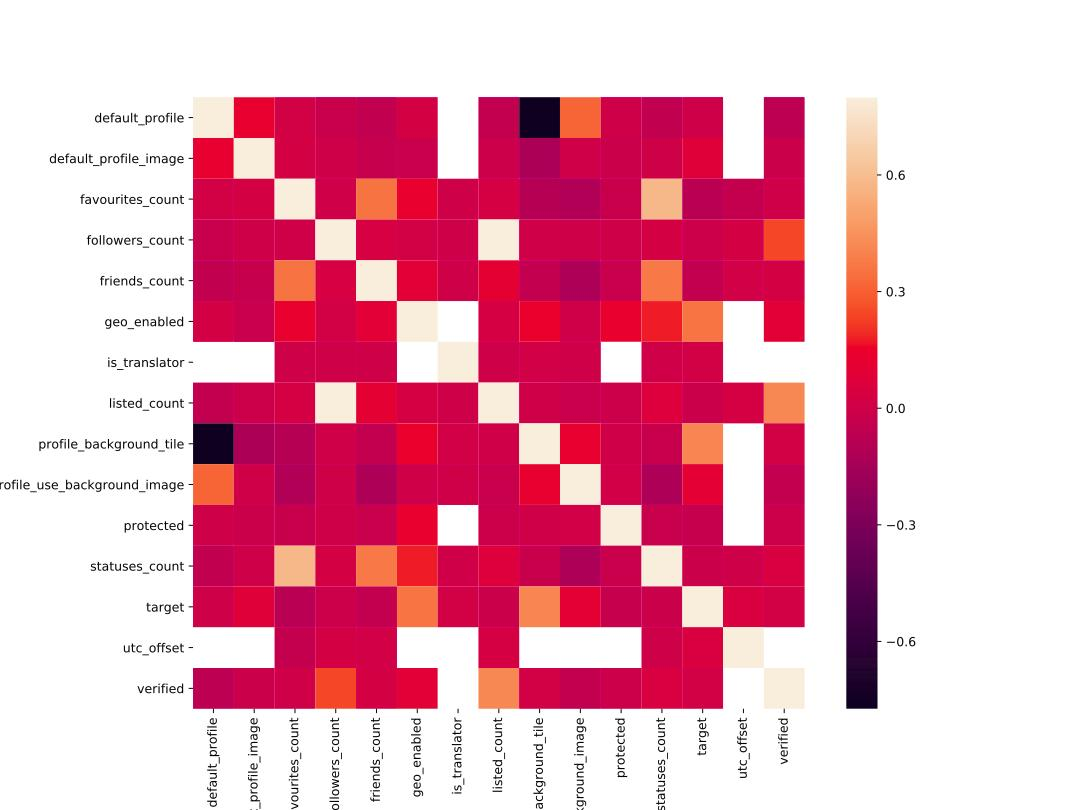
\includegraphics[width=\columnwidth]{chapter3/figure/heatmap.jpg}
	\caption{Heatmap that highlights the correlation between the features}
	\label{fig:heatmap}
\end{figure}

Moreover in figure (\ref{fig:msno}) it is possible to see the distribution of the missing values. This is fundamental for the features engineering step.

\begin{figure}
	\centering
	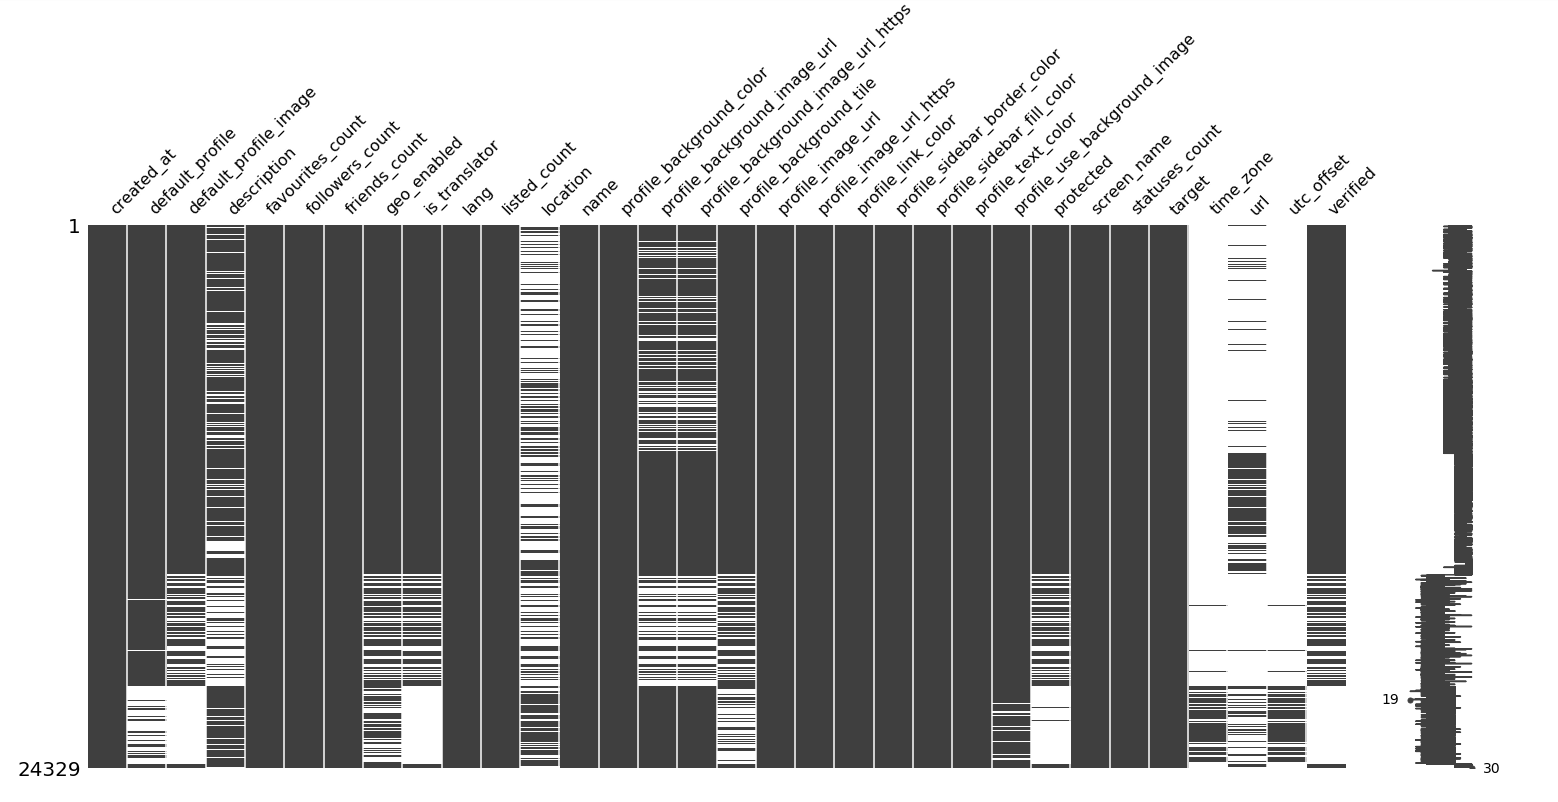
\includegraphics[width=\columnwidth]{chapter3/figure/msno.png}
	\caption{Missing values distribution for each feature}
	\label{fig:msno}
\end{figure}

\newpage
Finally we performed three further analyses. With the heatmap we could not detect which features were more important. Anyway, during the hand-labelling step, we understood that some of these features were instead very useful to identify a few classes of our dataset. These attributes are \emph{''followers\_count''}, \emph{''friends\_count''} and \emph{''statuses\_count''}. For each of them we plotted a box-plot. It is a method used to represent groups of numerical data through their quartiles. In Figure \ref{fig:box_statuses} we can analyze the statuses count (number of tweets) for each target. We collected up to 100 tweets for each user, so this chart is limited to 100. Here we can notice an interesting behaviour: News-Spreaders and Spam-Bots are the classes with more tweets, while Fake-Followers have fewer statuses. By reflecting on the gols of the bots, this result is exactly what we expected to see. In fact Fake-Followers don't need to tweet, they just need to exist, while other types of bots have to publish many statuses, to draw attention on their contents.

\begin{figure}
	\centering
	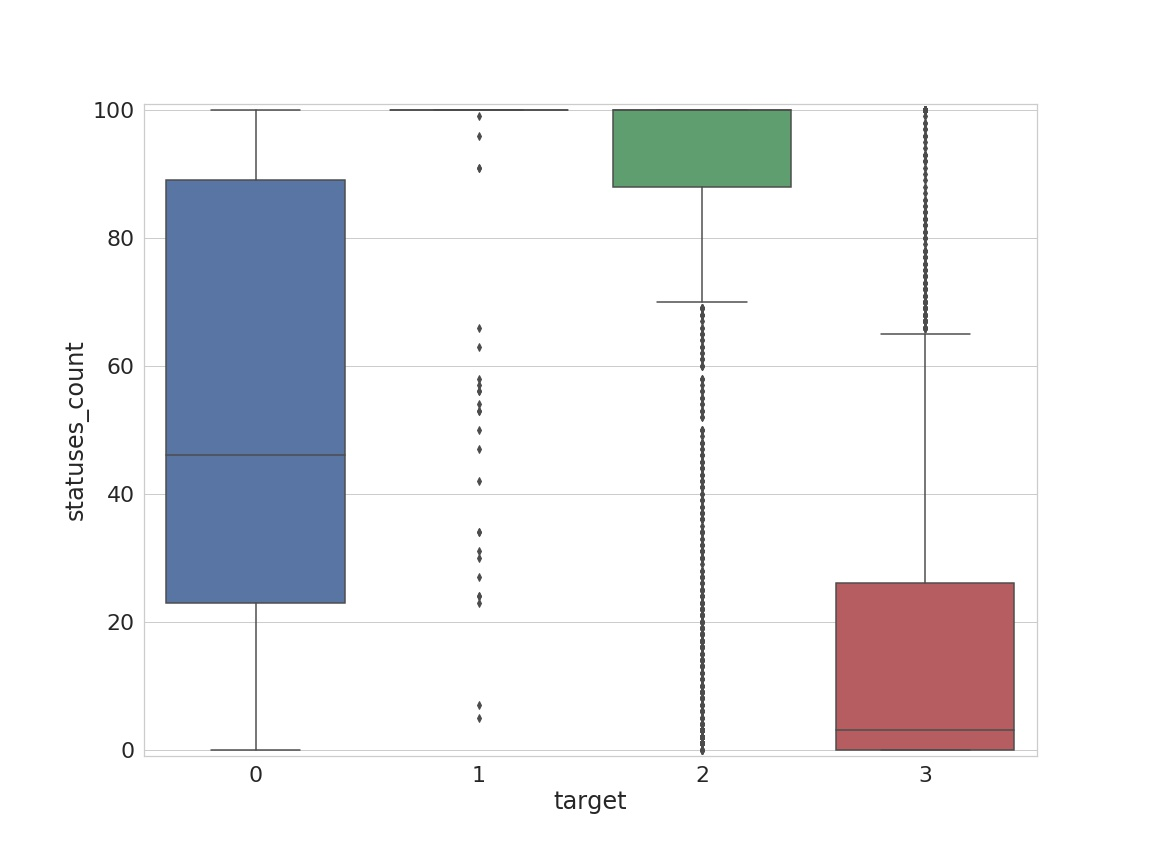
\includegraphics[width=\columnwidth]{chapter3/figure/boxplot.jpg}
	\caption{Boxplot statuses\_count}
	\label{fig:box_statuses}
\end{figure}
\newpage

\begin{figure}
	\centering
	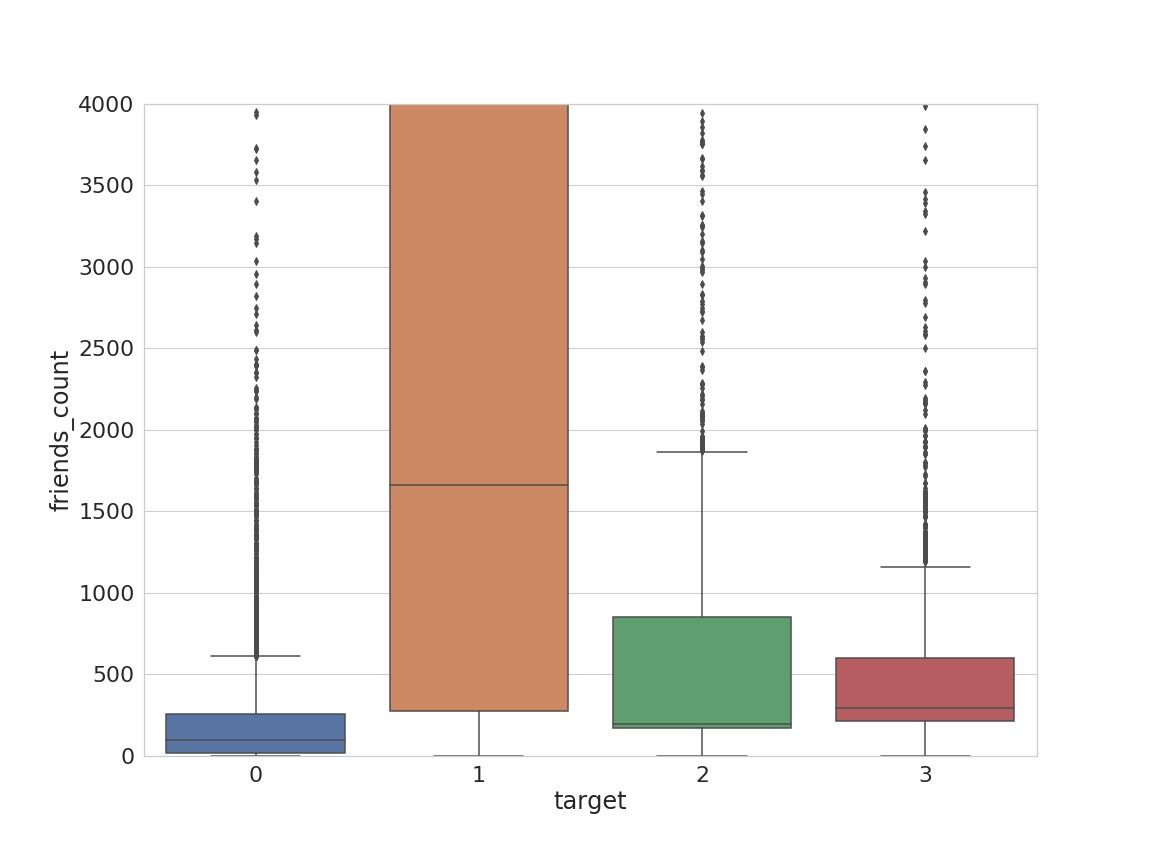
\includegraphics[width=\columnwidth]{chapter3/figure/boxplot_friends.jpg}
	\caption{Boxplot friends\_count}
	\label{fig:box_friends}
\end{figure}

\begin{figure}
	\centering
	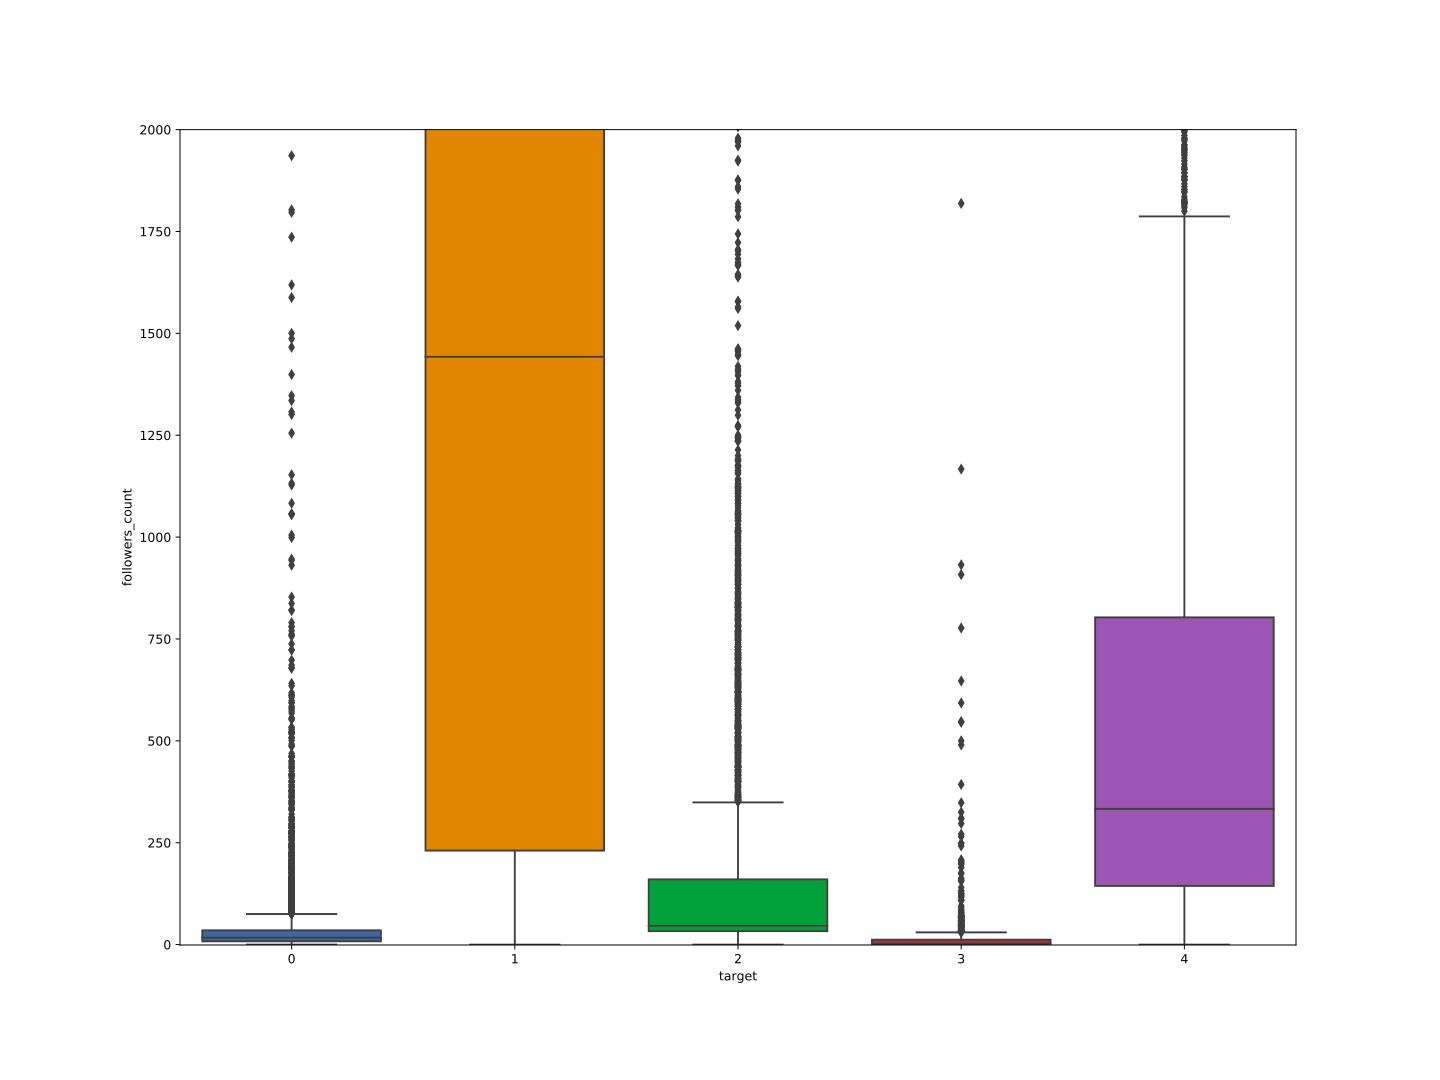
\includegraphics[width=\columnwidth]{chapter3/figure/boxplot_followers.jpg}
	\caption{Boxplot followers\_count}
	
	\label{fig:box_followers}
\end{figure}
In Figure \ref{fig:box_friends} and \ref{fig:box_followers} we performed the same analysis considering the \emph{''friends\_count''} and \emph{''followers\_count''} features. We limited the charts between 4,000 and 2,000 to keep them understandable. This two figures show us that News-Spreaders usually have a bigger network, while Fake-Followers just follow few users. News-Spreaders network may depends on the popularity of the news media. Other categories are more balanced and their differences can be attributed to the data and not to a different behaviuor between them.